\section{The (Human+AI)$^{2}$ Research Network}
\label{sec:network}

\begin{figure}[!t]
    \centering
    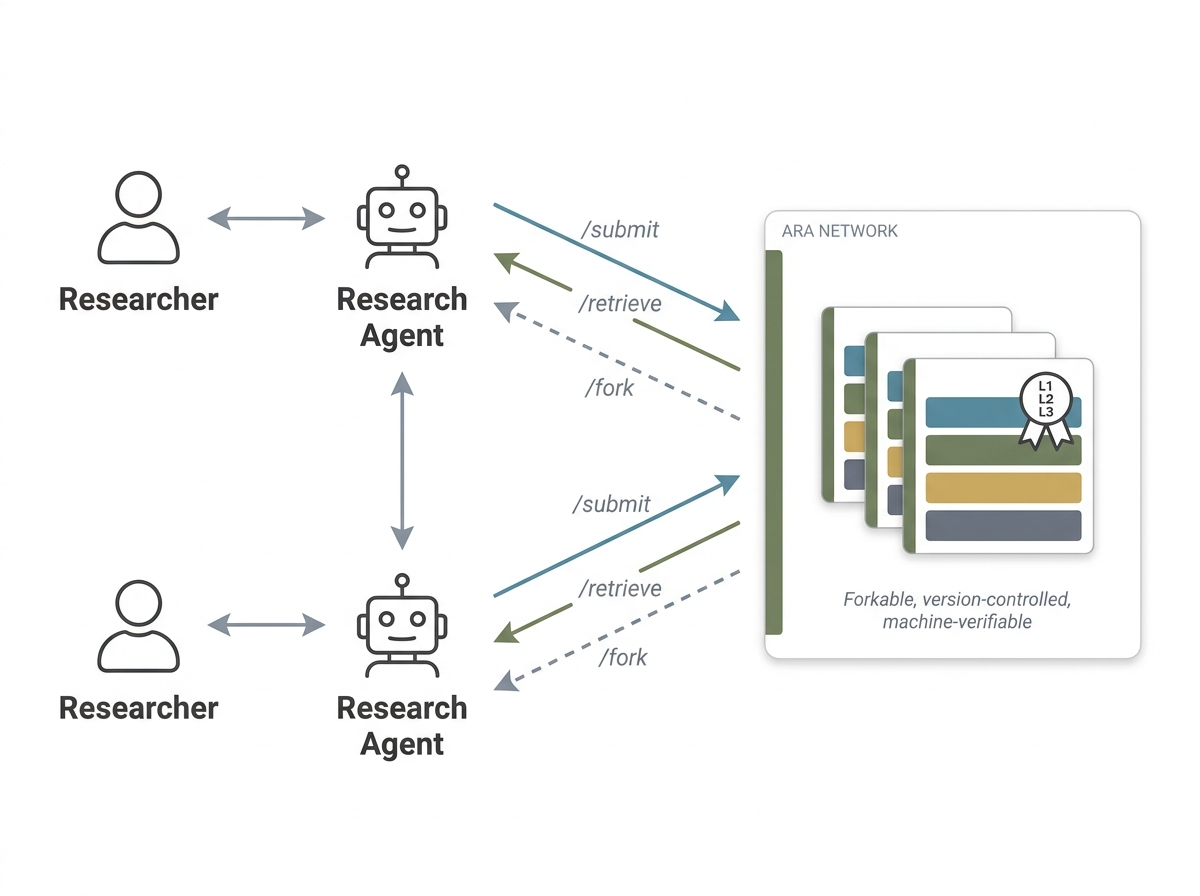
\includegraphics[width=0.85\linewidth]{figures/fig_human_ai_network.png}
    \caption{The (Human+AI)$^{2}$ research network. Each researcher works through a research agent that interfaces with a shared \ara{} network via \texttt{/submit}, \texttt{/retrieve}, and \texttt{/fork}; agents may also collaborate directly.}
    \label{fig:network}
\end{figure}

The previous sections describe the components of an \ara{}-native stack: the protocol (\S\ref{sec:protocol}), the Live Research Manager that captures work into the artifact during development (\S\ref{sec:live-pm}), the Compiler that imports the legacy literature (\S\ref{sec:ingestor}), and the Seal-gated review pipeline that verifies it (\S\ref{sec:review-system}). Composed, they form a scientific communication system whose primary object is no longer the static document but the \ara{} itself: a single canonical artifact that humans on each end direct agents to author, certify, render, and extend. We call the resulting structure a \textbf{(Human+AI)$^{2}$ network} (Figure~\ref{fig:network}).


On the producer side, researchers no longer work toward papers; they pursue questions, and the paper-as-output accrues automatically as an \ara{} along the way: the Live Research Manager folds each decision, dead end, and confirmed claim into the artifact during ordinary work, the Compiler imports legacy sources on demand, and at any milestone the artifact is routed through the Seal pipeline and registered publicly, where another team can fork a passing artifact, extend a claim, retain attribution to the parent, and submit the diff for re-review. 
On the consumer side, because the \ara{} is canonical, an agent renders it on demand into whatever surface the reader needs (paper, video, slides, interactive demo, or grounded dialogue), shaped by the reader's expertise, attention budget, and intent. 

With both ends agent-mediated and the artifact the only persistent state, contributions compound at the level of artifacts rather than sentences: publishing becomes a Git-like operation, reviewers consume Seal-attested artifacts through their preferred surfaces, and downstream agents read \ara{}s as structured baselines, training environments, or starting points for new questions. The result is a queryable scientific commons in which every contribution is an executable diff, and the cost of understanding, reproduction, and extension falls with each new artifact admitted rather than rising against it. \S\ref{sec:eval} asks whether today's agents can already operate this substrate; \S\ref{sec:discussion} maps near-, medium-, and long-term extensions.
